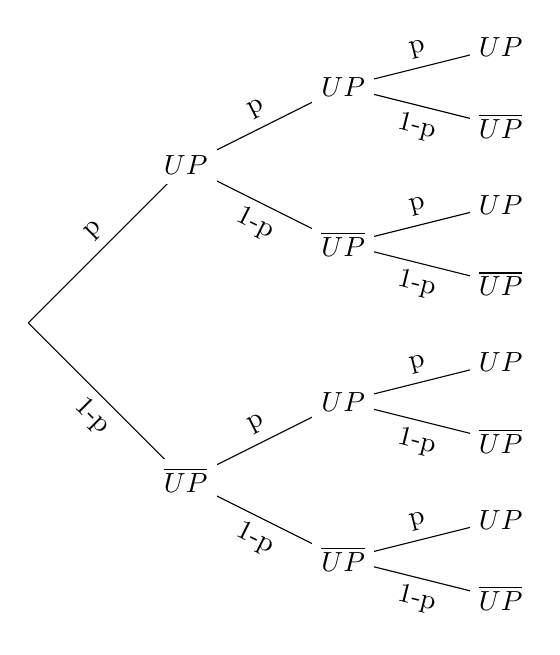
\begin{tikzpicture}[xscale=1,yscale=1]
\draw (0,0)--(-2,0.5) node[midway, below, sloped]{1-p};
\draw (0,1)--(-2,0.5) node[midway, above, sloped]{p};
\draw (0,2)--(-2,2.5) node[midway, below, sloped]{1-p};
\draw (0,3)--(-2,2.5) node[midway, above, sloped]{p};
\draw (0,4)--(-2,4.5) node[midway, below, sloped]{1-p};
\draw (0,5)--(-2,4.5) node[midway, above, sloped]{p};
\draw (0,6)--(-2,6.5) node[midway, below, sloped]{1-p};
\draw (0,7)--(-2,6.5) node[midway, above, sloped]{p};
\draw (-2,0.5)--(-4,1.5) node[midway, below, sloped]{1-p};
\draw (-2,2.5)--(-4,1.5) node[midway, above, sloped]{p};
\draw (-2,4.5)--(-4,5.5) node[midway, below, sloped]{1-p};
\draw (-2,6.5)--(-4,5.5) node[midway, above, sloped]{p};
\draw (-4,1.5)--(-6,3.5) node[midway, below, sloped]{1-p};
\draw (-4,5.5)--(-6,3.5) node[midway, above, sloped]{p};
\draw (0,0) node[fill=white]{$\overline{UP}$};
\draw (0,1) node[fill=white]{$UP$};
\draw (0,2) node[fill=white]{$\overline{UP}$};
\draw (0,3) node[fill=white]{$UP$};
\draw (0,4) node[fill=white]{$\overline{UP}$};
\draw (0,5) node[fill=white]{$UP$};
\draw (0,6) node[fill=white]{$\overline{UP}$};
\draw (0,7) node[fill=white]{$UP$};
\draw (-2,0.5) node[fill=white]{$\overline{UP}$};
\draw (-2,2.5) node[fill=white]{$UP$};
\draw (-2,4.5) node[fill=white]{$\overline{UP}$};
\draw (-2,6.5) node[fill=white]{$UP$};
\draw (-4,1.5) node[fill=white]{$\overline{UP}$};
\draw (-4,5.5) node[fill=white]{$UP$};
\end{tikzpicture}